\begin{center}
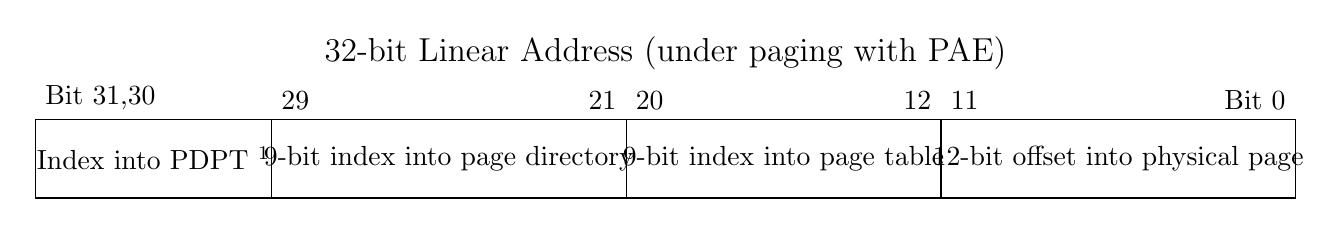
\begin{tikzpicture}
\draw (0,0) rectangle (3,1) node [pos = 0.5] {Index into PDPT \footnote{Page Directory Pointer Table}};
\draw (3,0) rectangle (7.5,1) node [pos = 0.5] {9-bit index into page directory};
\draw (7.5,0) rectangle (11.5,1) node [pos = 0.5] {9-bit index into page table};
\draw (11.5,0) rectangle (16,1) node [pos = 0.5] {12-bit offset into physical page};
\draw node at (0,1) [above right] {Bit 31,30};
\draw node at (3,1) [above right] {29};
\draw node at (7.5,1) [above left] {21};
\draw node at (7.5,1) [above right] {20};
\draw node at (11.5,1) [above left] {12};
\draw node at (11.5,1) [above right] {11};
\draw node at (16,1) [above left] {Bit 0};
\draw node at (8,1.5) [above] {{\large 32-bit Linear Address (under paging with PAE)}};
\end{tikzpicture}
\end{center}